\documentclass[xcolor=table, aspectratio=169]{beamer}

% !TEX engine = pdflatex
%\usepackage{arev}
\usepackage{amsmath,amssymb,amscd}
\usepackage{dsfont}
\usepackage{mathrsfs}
\usepackage{yfonts}
\usepackage{bm}
\usepackage{graphicx}
\usepackage{tabularx}
\usepackage{animate}
\usepackage{listings}
%\usepackage{mathtools}
%\usepackage{ifthen}

%\usepackage{xeCJK}
%\usepackage{fontspec}
%\newfontfamily\cjkfont{PingFang SC}
%\setCJKmainfont{PingFang SC}
\newcolumntype{x}{>{\centering\arraybackslash}X}
\renewcommand{\arraystretch}{1.5}
%\newcommand{\uone}{\mathrm U(1)}
\newcommand{\uone}{\mathbb R/\mathbb Z}
\DeclareMathOperator{\img}{img}
\DeclareMathOperator{\hhom}{Hom}
\DeclareMathOperator{\id}{id}
\usepackage{tikz}
	\usetikzlibrary{calc}
	\usetikzlibrary{arrows,shapes, positioning, matrix}
	\usetikzlibrary{decorations.markings}
	\tikzset{>=stealth}
	\tikzstyle arrowstyle=[scale=1]
	\tikzstyle directed=[postaction={decorate,decoration={markings,
 	   mark=at position .15 with {\arrow[arrowstyle]{stealth}}}}]
\tikzstyle string=[thick,postaction={decorate,decoration={markings,
    mark=at position .55 with {\arrow[arrowstyle]{stealth}}}}]
\tikzstyle dual_string=[dashed,postaction={decorate,decoration={markings,
    mark=at position .55 with {\arrow[arrowstyle]{stealth}}}}]

\tikzstyle dw=[thick,postaction={decorate,decoration={markings,
    mark=at position 1 with {\arrow[arrowstyle]{stealth}}}}]
\tikzstyle group=[mbg]
\newcommand*{\halfway}{0.5*\pgfdecoratedpathlength+.5*8pt}\tikzstyle arrowstyle=[scale=1]
\newcommand*{\halfwayb}{0.5*\pgfdecoratedpathlength}
\tikzstyle arrowstyle=[scale=1]
\tikzstyle fermion=[thick,postaction={decorate},decoration={markings,
    mark=at position \halfway with {\arrow[arrowstyle]{latex}}}]
\tikzstyle fermion2=[thick,postaction={decorate},decoration={markings,
        mark=at position \halfwayb with {\arrow[arrowstyle]{latex}}}]
\usepackage{tikz-cd}
\usepackage{pgffor}

\DeclareMathOperator{\tr}{Tr}
\DeclareMathOperator{\im}{Im}
\DeclareMathOperator{\re}{Re}

\mode<presentation>
{
  %\usetheme{Warsaw}
  % or ...
  %\useoutertheme{rectangle}
  \setbeamertemplate{frametitle}[default][center]
  \defbeamertemplate{itemize item}{flat}{\begin{pgfpicture}{-1ex}{0ex}{1ex}{2ex}
      \pgfpathcircle{\pgfpoint{0pt}{.6ex}}{0.6ex}
      \pgfusepath{fill}
    \end{pgfpicture}%
  }
  \defbeamertemplate{itemize subitem}{flat}{\footnotesize\raise0.5pt\hbox{\textbullet}}
  \defbeamertemplate{itemize subsubitem}{flat}{\footnotesize\raise0.5pt\hbox{\textbullet}}

  %\useinnertheme{circles}
  \setbeamertemplate{items}[flat]
  \setbeamertemplate{sections/subsections in toc}[circle]
  \setbeamertemplate{blocks}[rounded]
  \setbeamertemplate{title page}[default][colsep=-4bp,rounded=true]
  \setbeamertemplate{part page}[default][colsep=-4bp,rounded=true]
  \setbeamercovered{transparent}
  %\usecolortheme{spruce}
  %\definecolor{THU}{RGB}{116,61,130}
  \definecolor{mbg}{RGB}{0,0,160}
  \setbeamercolor*{palette primary}{fg=white,bg=mbg}
  \setbeamercolor*{titlelike}{parent=palette primary}
  \setbeamercolor*{structure}{fg=mbg}
  \setbeamercolor{frametitle}{fg=white,bg=mbg}
  % or whatever (possibly just delete it)
  \setbeamercolor{block title}{bg=mbg,fg=white}
  \setbeamercolor{block body}{bg=mbg!15}


  \addtobeamertemplate{navigation symbols}{}{ \hspace{1em}%
    \usebeamerfont{footline}%
    \insertframenumber / \inserttotalframenumber }
}


%\usepackage[english]{babel}
% or whatever

%\usepackage[latin1]{inputenc}
% or whatever

%\usepackage{times}
%\usepackage[T1]{fontenc}
% Or whatever. Note that the encoding and the font should match. If T1
% does not look nice, try deleting the line with the fontenc.

\title[Intro to SptSet] % (optional, use only with long paper titles)
{SptSet: A GAP package for computing fermionic SPT classification and beyond}

\author[Y Qi] % (optional, use only with lots of authors)
{Yang~Qi}
% - Give the names in the same order as the appear in the paper.
% - Use the \inst{?} command only if the authors have different
%   affiliation.

\institute[Fudan] % (optional, but mostly needed)
{Department of Physics, Fudan University}
% - Use the \inst command only if there are several affiliations.
% - Keep it simple, no one is interested in your street address.

%\date{2016 Annual Meeting of Fudan CFTPP} % (optional, should be abbreviation of conference name)
%{Fudan University, Oct 13 2015}
\date{Shenzhen Forum on Strongly-Correlated Systems, Jan. 2020.}
% - Either use conference name or its abbreviation.
% - Not really informative to the audience, more for people (including
%   yourself) who are reading the slides online

\subject{Theoretical Physics}
% This is only inserted into the PDF information catalog. Can be left
% out.




% If you have a file called "university-logo-filename.xxx", where xxx
% is a graphic format that can be processed by latex or pdflatex,
% resp., then you can add a logo as follows:

\pgfdeclareimage[height=1cm]{university-logo}{../resources/fudan}
\logo{\pgfuseimage{university-logo}}

\AtBeginSection[]
{
  \begin{frame}<beamer>{Outline}
			\tableofcontents[currentsection,currentsubsection]
			%\begin{center}
			%	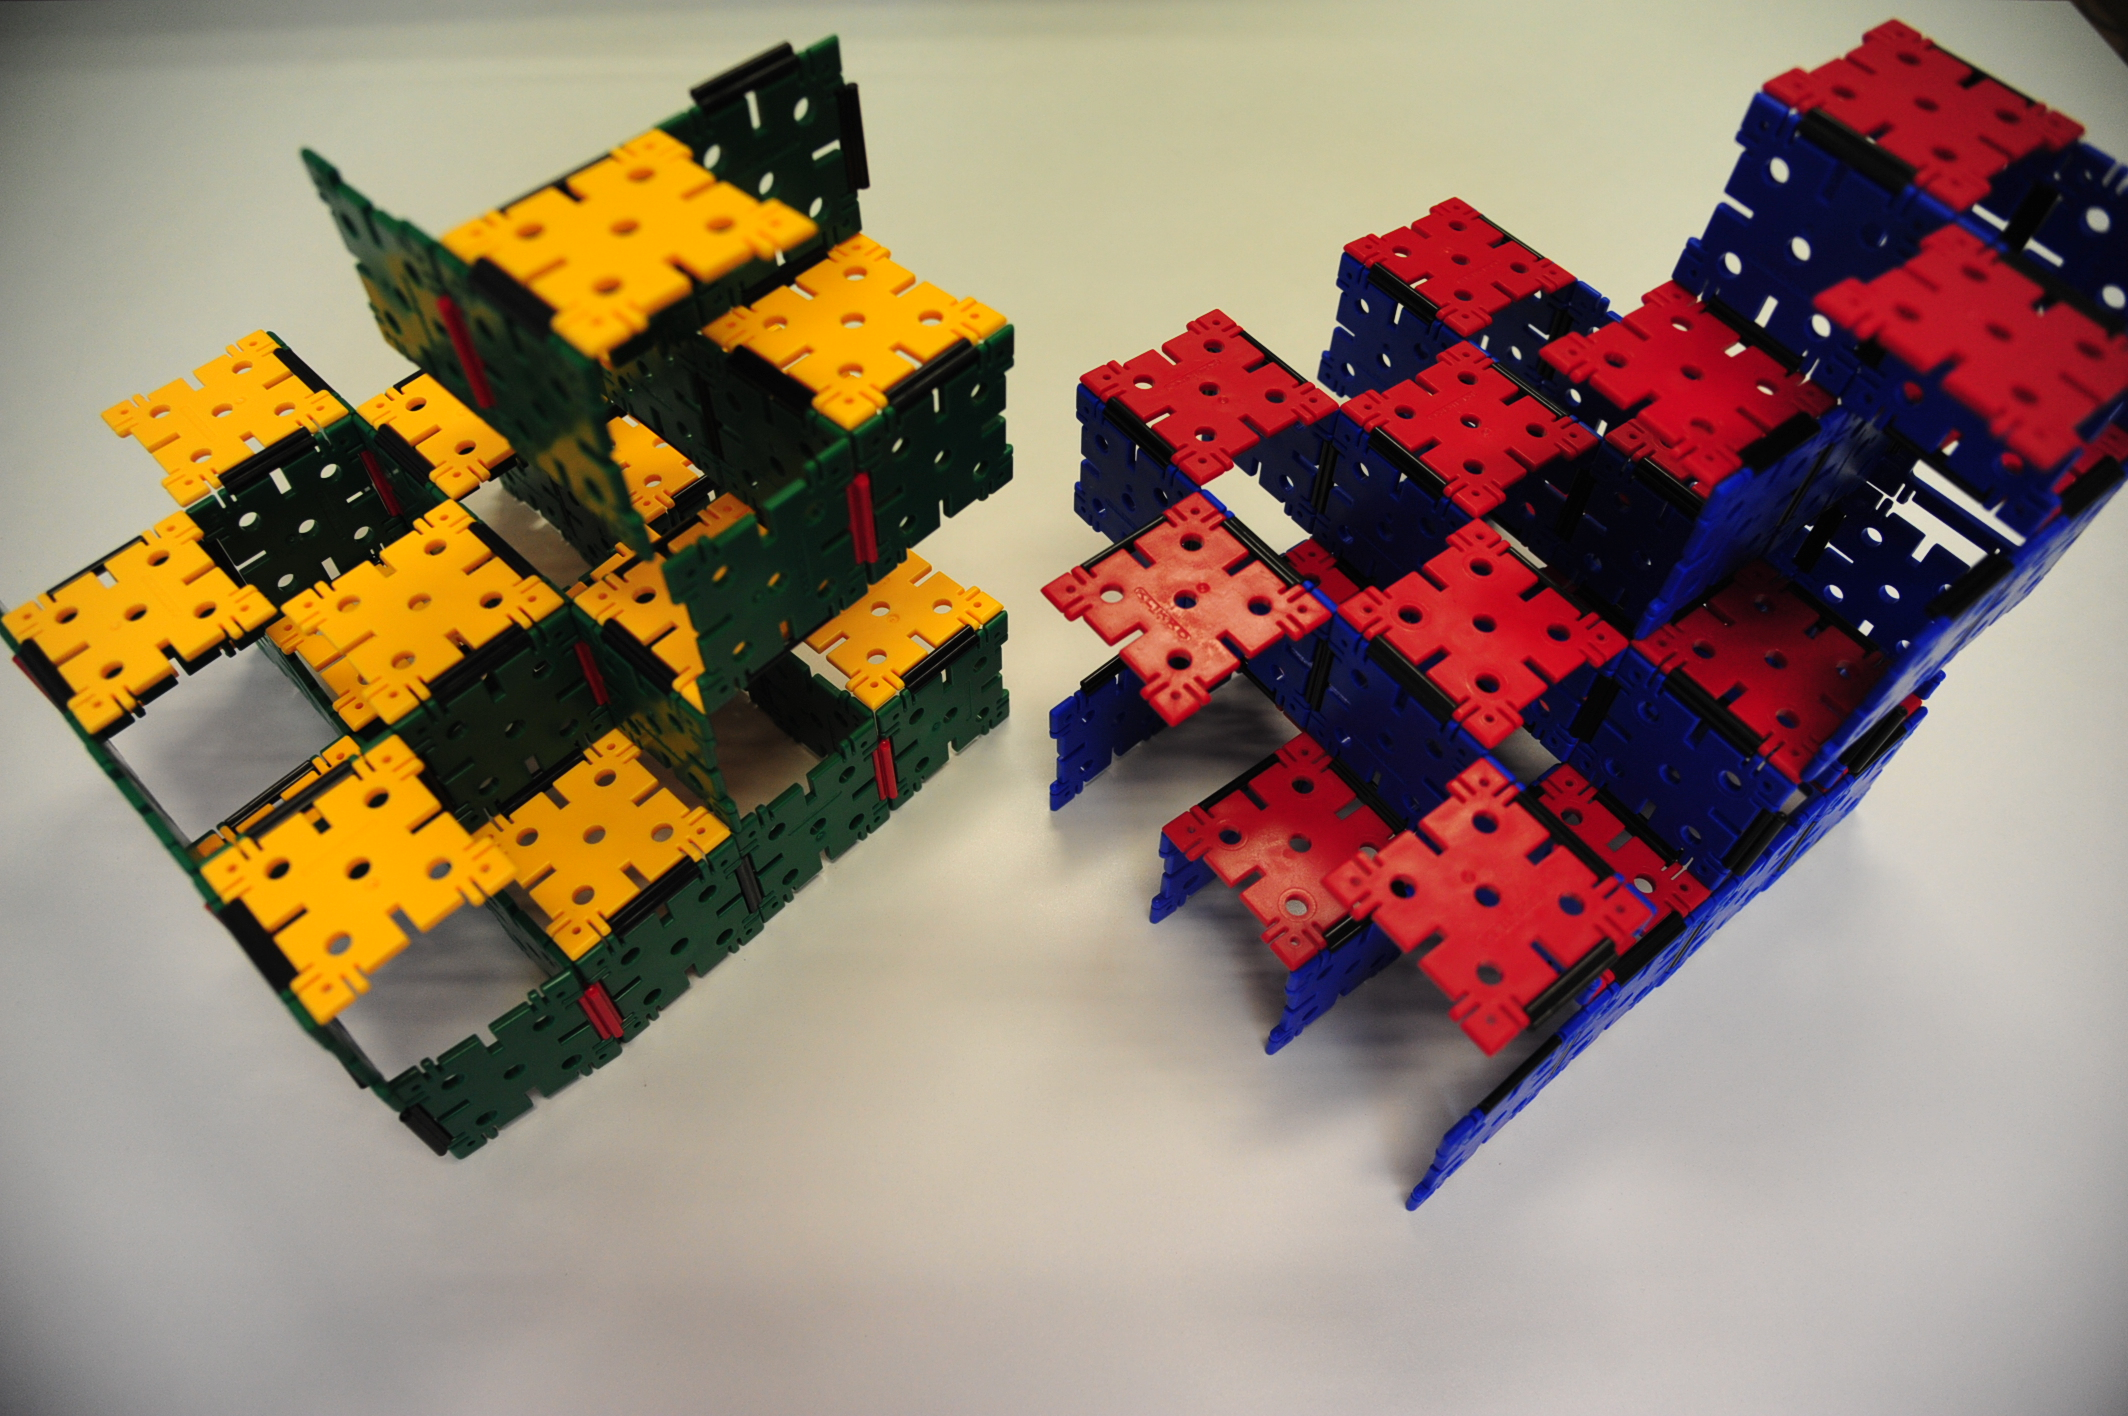
\includegraphics[height=4cm]{toys}
			%\end{center}
  \end{frame}
}


% Delete this, if you do not want the table of contents to pop up at
% the beginning of each subsection:

\begin{document}

\begin{frame}
  \titlepage
\end{frame}

\begin{frame}{Collaborators}
\begin{itemize}
%\item Yunqing Ouyang (欧阳云卿): Fudan University.
%\item Qing-Rui Wang (王晴睿): Chinese University of Hong Kong $\rightarrow$ Yale University.
%\item Zheng-Cheng Gu (顾正澄): Chinese University of Hong Kong.
\item Yunqing Ouyang: Fudan University.
\item Qing-Rui Wang: Chinese University of Hong Kong $\rightarrow$ Yale University.
\item Zheng-Cheng Gu: Chinese University of Hong Kong.
\begin{center}
	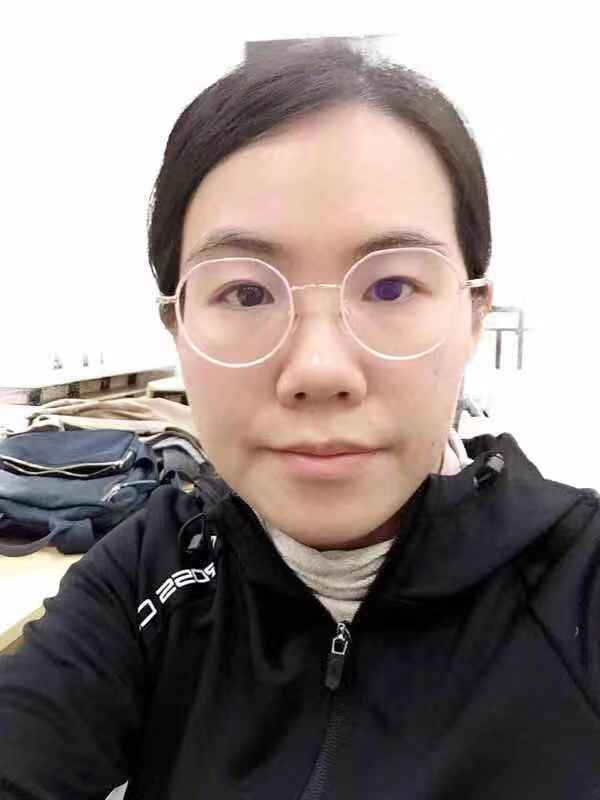
\includegraphics[height=3cm]{../people/yunqing}
	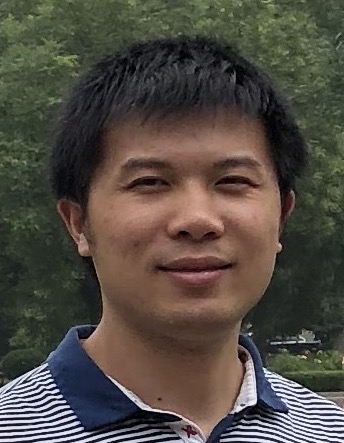
\includegraphics[height=3cm]{../people/qingrui}
	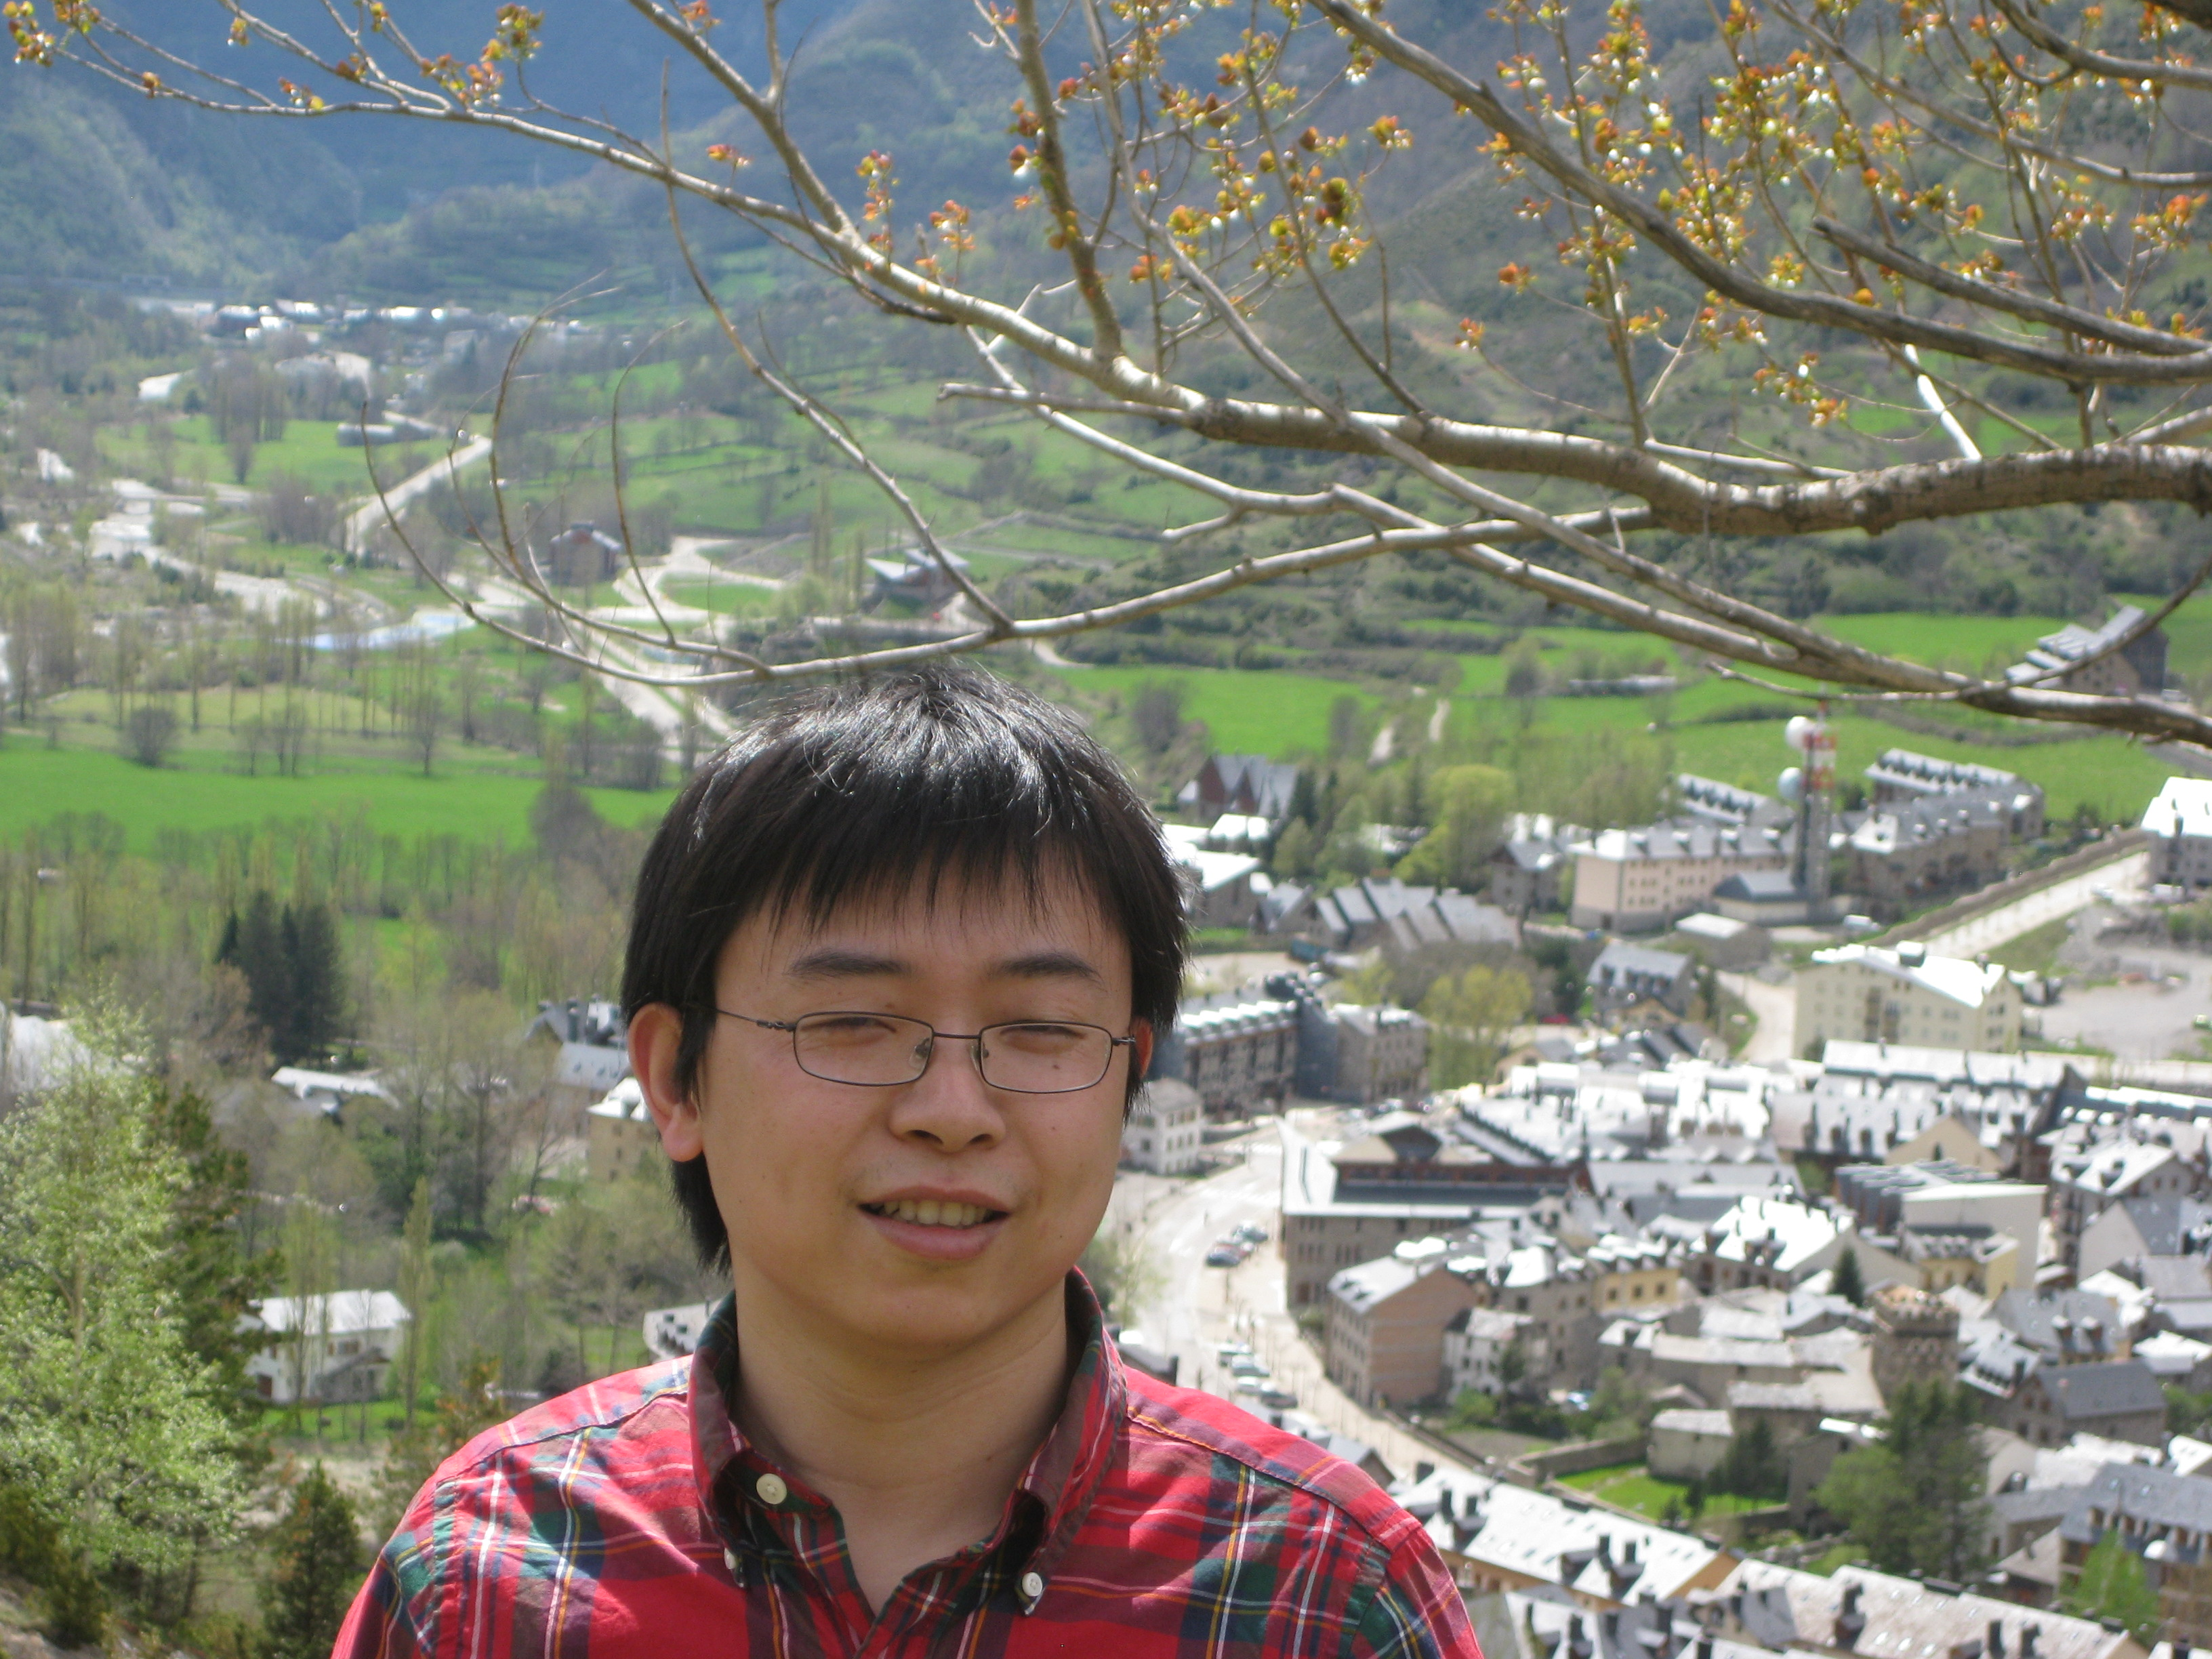
\includegraphics[height=3cm]{../people/zhengcheng}
\end{center}
\item Yunqing Ouyang, Qing-Rui Wang, Zheng-Cheng Gu and YQ, to appear.
\end{itemize}
\end{frame}

\section{Demo: GAP, HAP and SptSet.}

\begin{frame}[fragile]
\frametitle{GAP}
\begin{itemize}
\item GAP = Group, Algorithm and Programming.
\item \url{www.gap-system.org}
\item Easy to create and study groups.
\end{itemize}

\begin{lstlisting}[basicstyle=\footnotesize]
gap> G := CyclicGroup(4);
pc group of size 4 with 2 generators>
gap> G := DihedralGroup(6);
pc group of size 4 with 2 generators>
gap> G := SpaceGroupBBNWZ(3, 12);
\end{lstlisting}

\end{frame}

\begin{frame}[fragile]
	\frametitle{HAP and group cohomology}
	\begin{itemize}
		\item bSPT: $H^D[G,\uone]$ can be computed directly using HAP in GAP.
		\item $H^D[G,\uone]$ ``='' $H^{D+1}[G,\mathbb Z]$. \emph{See X-G Wen, PRB \textbf{91}, 205101 (2015)}
	\end{itemize}
	\begin{columns}
		\column{.5\columnwidth}
	\begin{lstlisting}[basicstyle=\footnotesize]
gap> LoadPackage("HAP");
gap> G := CyclicGroup(4);
pc group of size 4 with 2 generators>
gap> GroupCohomology(G, 2);
[ 4 ]
gap> GroupCohomology(G, 3);
[  ]
gap> GroupCohomology(G, 4);
[ 4 ]
gap> GroupCohomology(G, 5);
[  ]
\end{lstlisting}
	\column{.5\columnwidth}
	\[H^{2n+1}[\mathbb Z_4,\uone] = \mathbb Z_4\]
	\[H^{2n}[\mathbb Z_4,\uone] = \mathbb Z_1\]
	\end{columns}
\end{frame}

\begin{frame}[fragile]
	\frametitle{Implimenting chain maps in GAP}
	\begin{itemize}
		\item We are working on a GAP package to impliment the chain maps and to compute fSPT classifications.
		\item User only need to input the mappingin terms of inhomogeneous cocycles.
		\item The package automatically computes the mapping using the simplified resolution.
	\end{itemize}
\begin{lstlisting}[basicstyle=\footnotesize,morekeywords={function,return,local,if,fi,then,end},showspaces=false,showtabs=false, keywordstyle=\color{blue}]
SptSetInstallCoboundary(ss, 2, 2, 1,
function(n2, dn2)
  return function(g1, g2, g3, g4)
    local val;
    val := 1/2 * (n2(g1, g2) * n2(g3, g4) mod 2);
    if dn2 <> ZeroCocycle@ then
      val := val + 1/2 * ((n2(g1*g2*g3, g4) * dn2(g1, g2, g3)
        + n2(g1, g2*g3*g4) * dn2(g2, g3, g4)) mod 2);
      val := val + 1/2 * (dn2(g1, g2, g3*g4) * dn2(g1*g2, g3, g4) mod 2);
      val := val - 1/4 * (dn2(g1, g2, g3) * (1 - dn2(g1, g2, g3*g4)) mod 2);
    fi;
    return val;
  end;
end);
\end{lstlisting}
\end{frame}

\begin{frame}[fragile]
	\frametitle{Example: computing fSPT}
	Consider 2D fSPT, $G=\mathbb Z_4$:
\begin{lstlisting}[basicstyle=\footnotesize]
gap> LoadPackage("SptSet");;
gap> G := CyclicGroup(4);;
gap> R := ResolutionFiniteGroup(G, 6);;
gap> utAct := SptSetTrivialGroupAction(G);;
gap> ss := FermionEZSPTSpecSeq(R, utAct);;
gap> FermionSPTLayers(ss, 2);
[ <ZL-Module with torsions [ 2 ]>, <ZL-Module with torsions [ 2 ]>,
  <ZL-Module with torsions [ 4 ]> ]
gap> z2tAct := GroupHomomorphismByImagesNC(G, GL(1, Integers),
>   GeneratorsOfGroup(G), [ [[-1]], [[1]] ]);;
gap> ss := FermionEZSPTSpecSeq(R, z2tAct);;
gap> FermionSPTLayers(ss, 2);
[ <ZL-Module with torsions [ 2 ]>, <ZL-Module []>, <ZL-Module []> ]
\end{lstlisting}

Example: compute fSPT for 2D wallpaper groups.
\end{frame}

\begin{frame}
	\frametitle{Summary}
	\begin{itemize}
		\item Use a simplified free resolution to accelerate computation of group cohomology.
		\item Use chain maps between resolutions to compute maps between cohomology groups.
		\item We are working on a GAP package SptSet.
		\item Takes 5min to compute 2D fSPTs for all 17 wallpaper groups.
		\item Email me at \url{qiyang@fudan.edu.cn} for early access.
		\item We also have a program written in python: faster but much harder to use.
		\item Will add more functions (fSPT with nontrivial group extension, group structure, ...), tweak the performence, and publish.
	\end{itemize}
\end{frame}

\end{document}
